% author: Thorben Casper
% created on: 2020/03/11

\documentclass{elsarticle}

\usepackage[utf8]{inputenc}
\usepackage{subcaption}
\usepackage{amsmath}
\usepackage{graphicx}
\graphicspath{{./images}}
\usepackage[english]{babel}
\usepackage{tikz}
\usepackage{pgfplots}
\pgfplotsset{compat=1.15}
\usepackage[mode=buildnew]{standalone}
\usepackage{booktabs}
\usepackage{hyperref}
\usepackage{lipsum}
\usepackage{comment}
\usepackage{algorithm2e}
\newtheorem{remark}{Remark}[section]

% Load acronyms and new commands
\usepackage{glossaries}
\newacronym{cad}{CAD}{computer-aided design}
\makeglossaries

% user-defined macros
\usepackage[myoption]{my-macros}
\usepackage{macros-private}

\begin{document}

\begin{frontmatter}
\title{Example 01}
\author[address1,address2]{Author 1\corref{mycorrespondingauthor}}
\cortext[mycorrespondingauthor]{Corresponding author}
\ead{email1}
\author[address2]{Author 2}
\author[address2,address3]{Author 3}
\address[address1]{Address 1}
\address[address2]{Address 2}
\address[address3]{Address 3}
\begin{abstract}
This is an example paper to demonstrate the capabilities of flattenPaper.
\end{abstract}
\begin{keyword}
flatten, figures, bibliography
\end{keyword}
\end{frontmatter}

\section{Introduction}
\label{sec:introduction}

To provide an example using natbib, we use citations here~\cite{Jackson,Moore}.
In the following, the \emph{lipsum} package is exploited.

\lipsum[1-4]

\begin{figure}
    \centering
    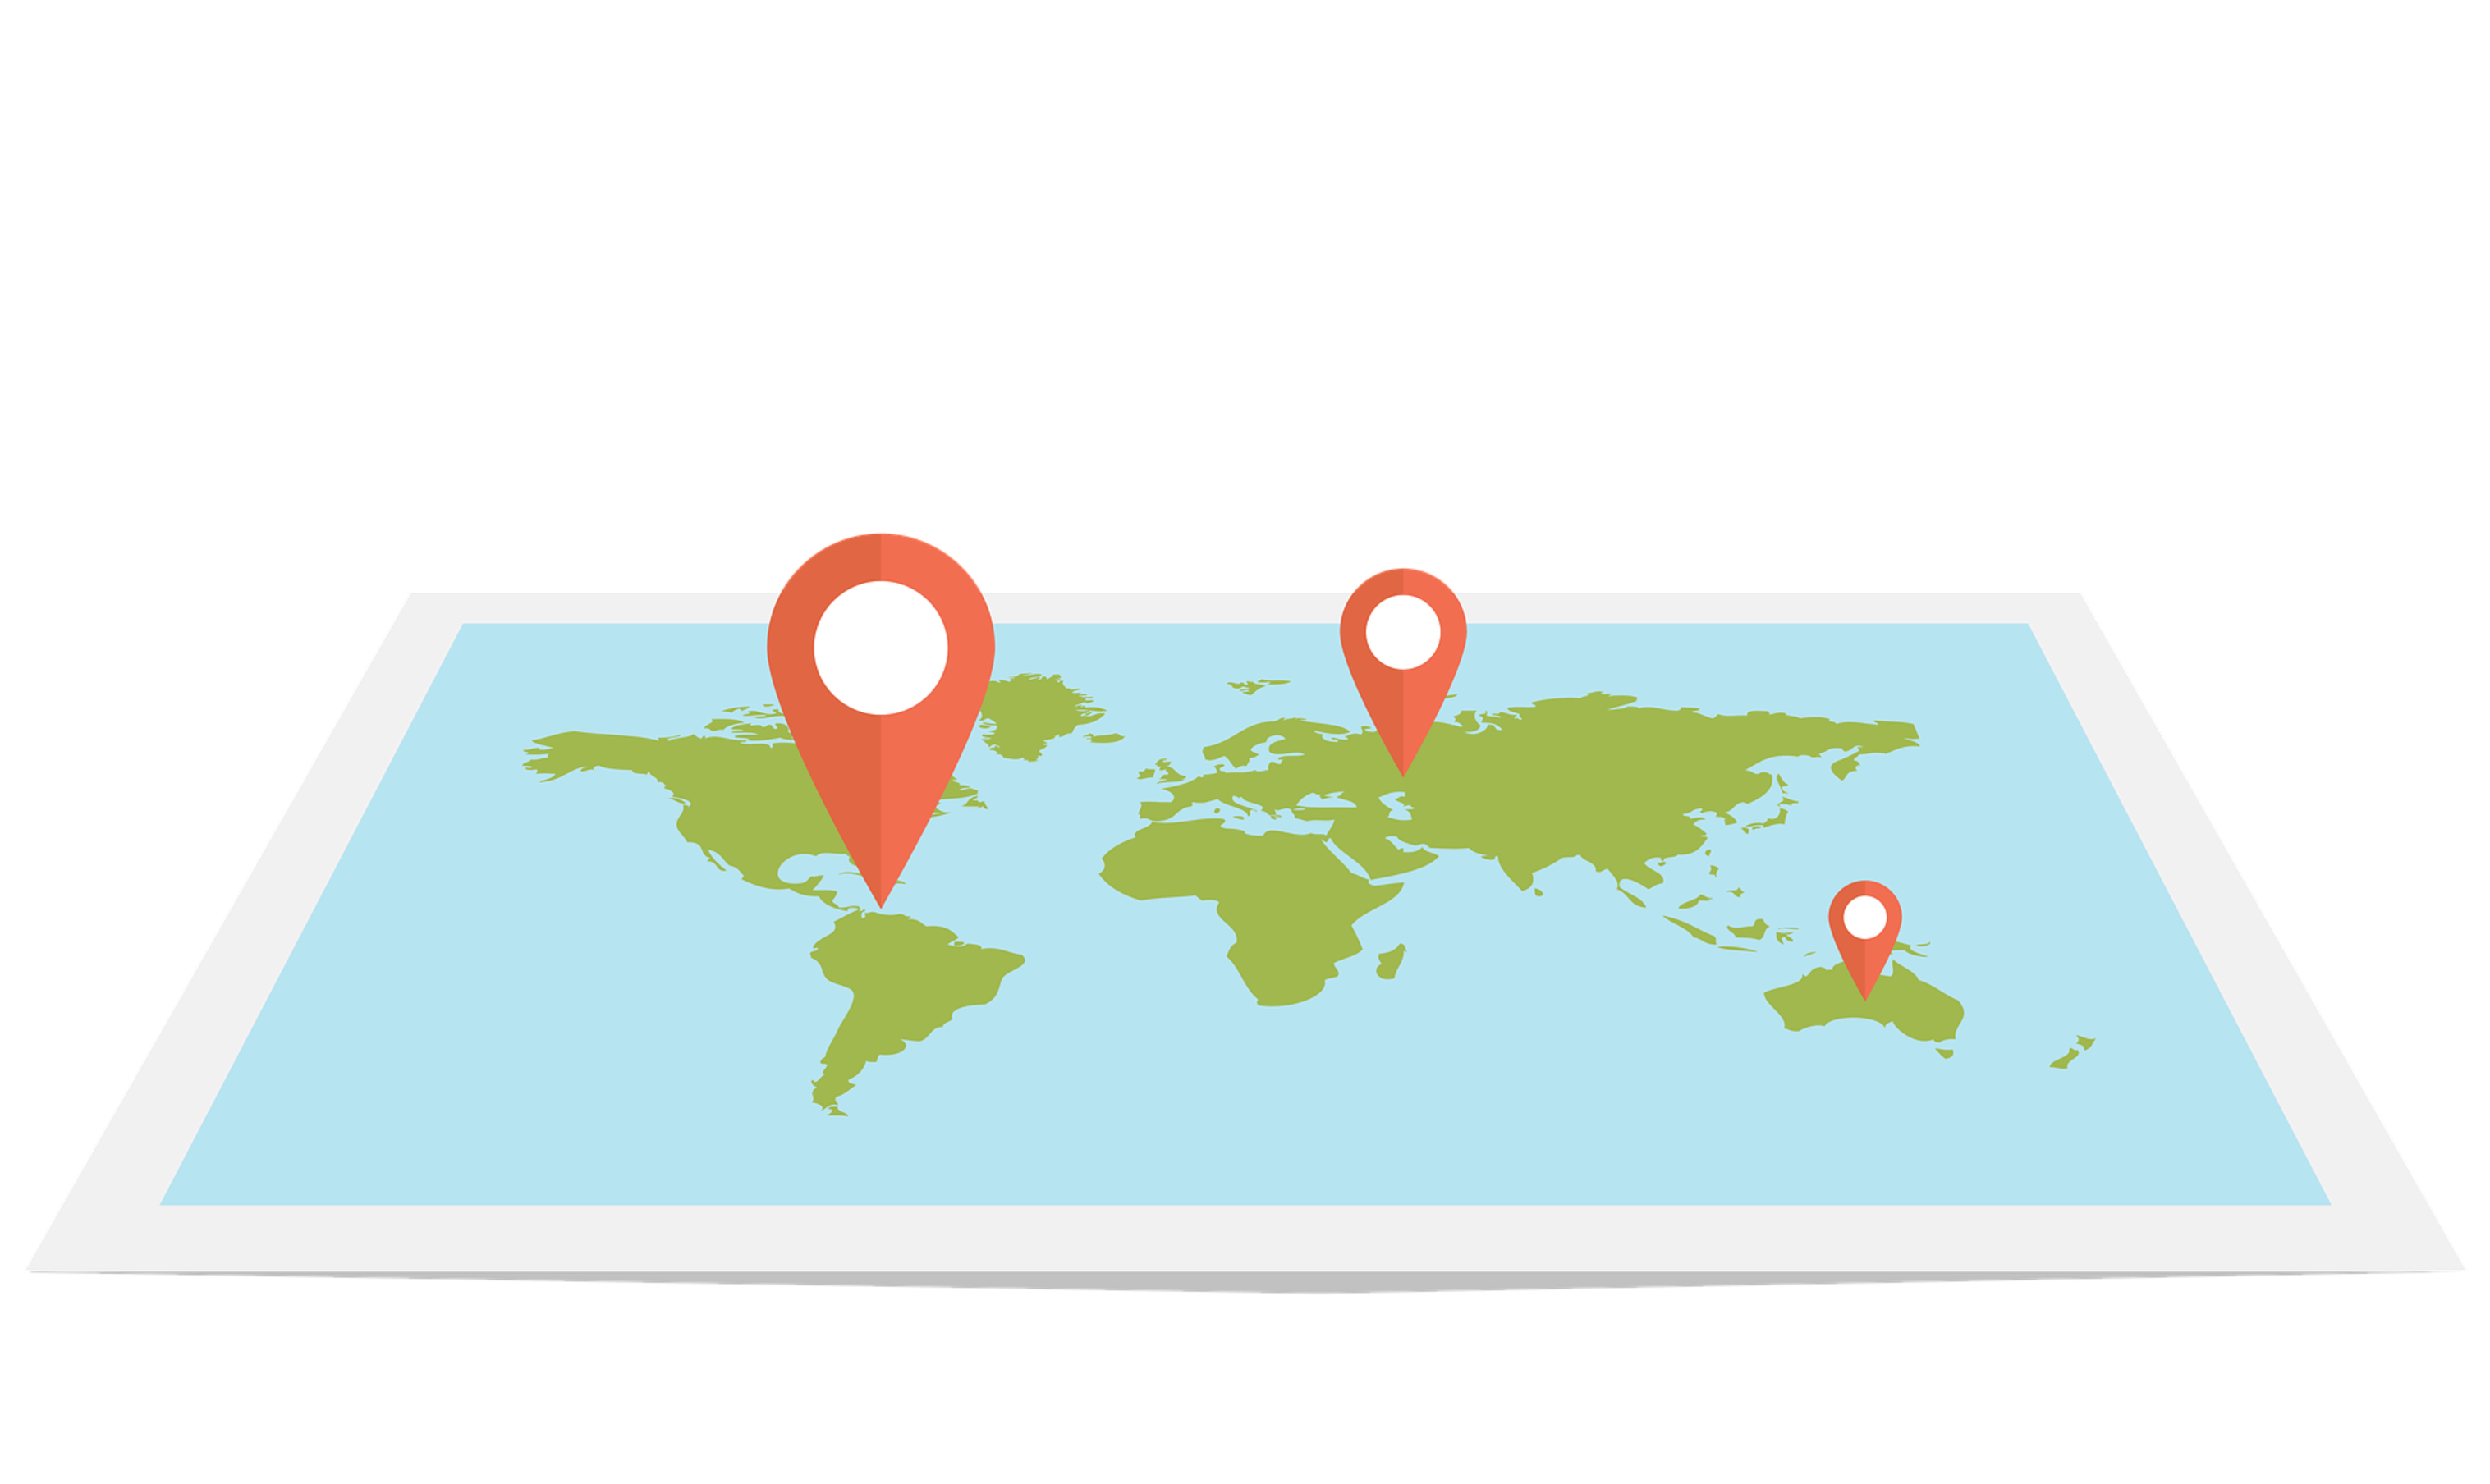
\includegraphics[width=0.4\columnwidth]{./figs/flatEarthEPS}
    \caption{An .eps-graphic using \emph{includegraphics}.}
    \label{fig:flatEarthEPS}
\end{figure}

\lipsum[5-6]

\begin{figure}
    \centering
    \begin{tikzpicture}
        \node at (0,0) {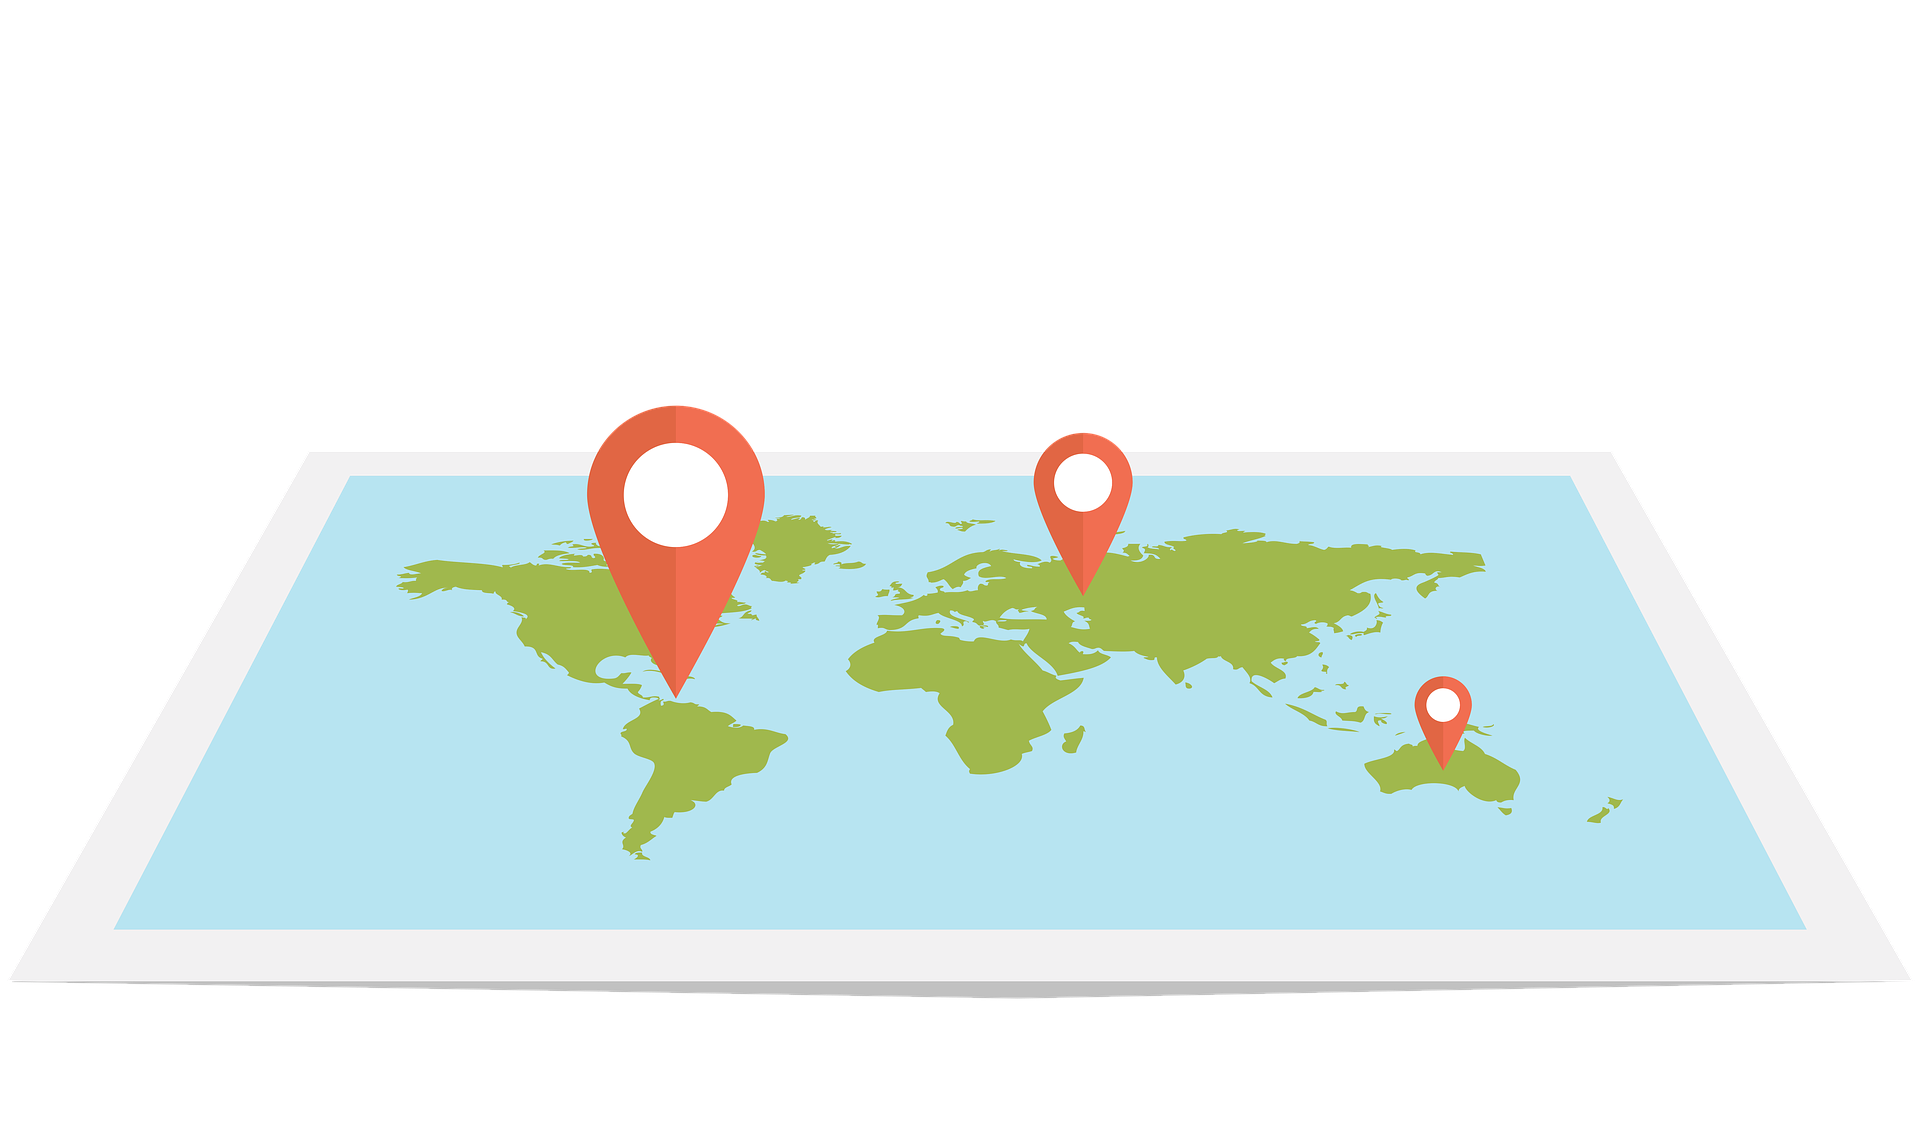
\includegraphics[width=0.6\textwidth]{./figs/flatEarthPNG}};
        \draw[->,ultra thick] (-1,1) -- (0.5,0);
    \end{tikzpicture}
    \caption{A .png-graphic using \emph{includegraphics} inside a \emph{tikz} node.}
 \label{fig:flatEarthPNGinTIKZ}
\end{figure}

\lipsum[7-10]

\begin{figure}
    \centering
    \begin{tikzpicture}
        \node at (0,0) {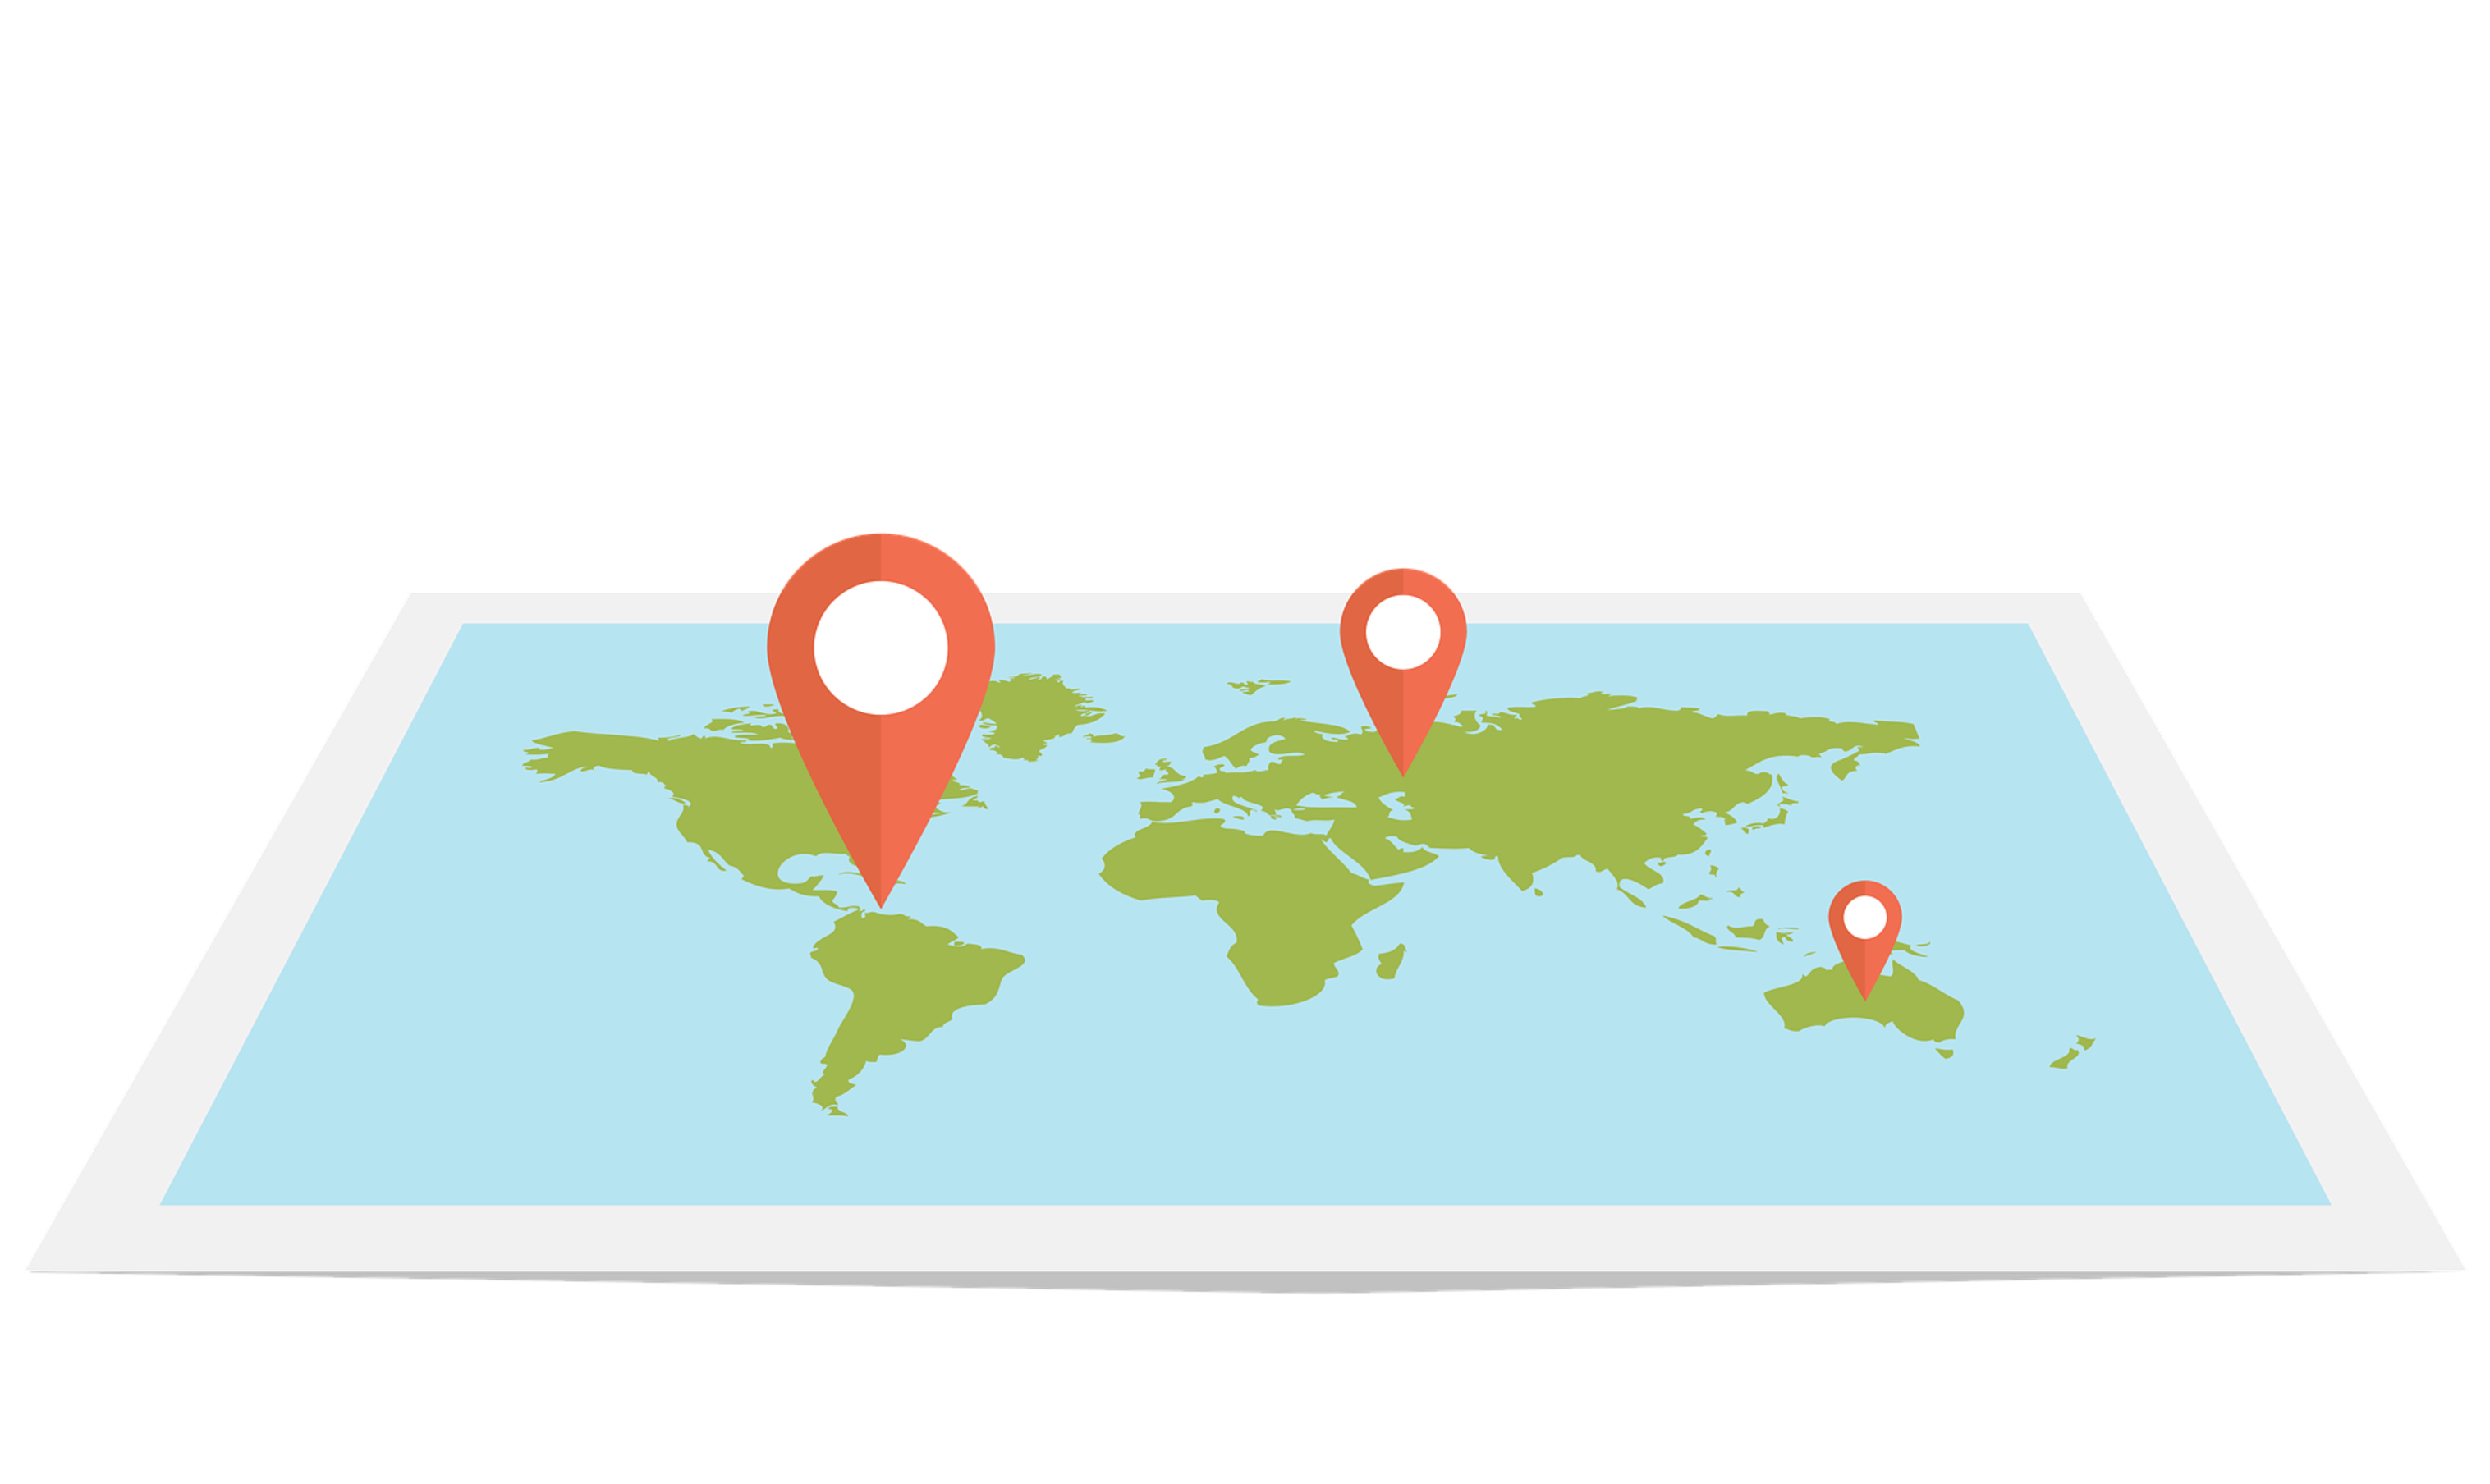
\includegraphics[width=0.6\textwidth]{./figs/flatEarthEPS}};
        \draw[->,ultra thick] (-1,1) -- (0.5,0);
    \end{tikzpicture}
    \caption{An .eps-graphic using \emph{includegraphics} inside a \emph{tikz} node.}
 \label{fig:flatEarthEPSinTIKZ}
\end{figure}

\lipsum[11]

\begin{figure}
    \centering
    \includestandalone{./images/circleDashed}
    \caption{A simple figure representing a dashed circle.}
    \label{fig:circleDashed}
\end{figure}

\lipsum[12]

%!TEX TS-program = pdflatex
%!TEX root = example02.tex

\section{Main Part}

\lipsum[11-13]

% an equation
\begin{equation}
    \Mmat = \Rmat
\end{equation}

% a simple figure
\begin{figure}[t]
    \centering
    \includestandalone{./images/matrix}
    \caption{A simple figures including the use of macros to typeset a matrix \Mmat.}
    \label{fig:matrix}
\end{figure}

\lipsum[14-15]

% subfigures using the subcaption package
\begin{figure}[t]
    \centering
    \begin{subfigure}[b]{0.49\textwidth}
        \centering
        \begin{tikzpicture}
    \draw(1,1) rectangle (5,5);
\end{tikzpicture}

        \caption{A simple square.}
        \label{fig:squareSimple}
    \end{subfigure}
    \begin{subfigure}[b]{0.49\textwidth}
        \centering
        \includestandalone{./figs/squareFilled}
        \caption{A filled square.}
        \label{fig:squareFilled}
    \end{subfigure}
    \caption{Using the \emph{subcaption} package to draw a simple and a filled square.}
    \label{fig:squares}
\end{figure}

\lipsum[16-17]

% a simple table
\begin{table}[t]
    \centering
    \begin{tabular}{ccc}\toprule
        Column 1 & Column 2 & Column 3\\\bottomrule\toprule
        Entry 1  & Entry 2  & Entry 3 \\\bottomrule
    \end{tabular}
    \caption{A simple table.}
    \label{tab:table}
\end{table}

\lipsum[17-18]

% subfigures using pgfplots and the subcaption package
\begin{figure}
    \centering
    \begin{subfigure}[b]{0.49\textwidth}
        \begin{tikzpicture}
            \begin{axis}[width=\columnwidth,xlabel=$x$,ylabel=$y$]
                \addplot{x};
            \end{axis}
        \end{tikzpicture}
    \end{subfigure}
    \begin{subfigure}[b]{0.49\textwidth}
        \begin{tikzpicture}
            \begin{axis}[width=\columnwidth,xlabel=$x$,ylabel=$y$]
                \addplot{x^2};
            \end{axis}
        \end{tikzpicture}
    \end{subfigure}
    \caption{Using the \emph{subcaption} package to draw simple pgfplot environments plotting $y=x$ and $y=x^2$.}
    \label{fig:pgfplot}
\end{figure}

\lipsum[18-19]

% an algorithm
\begin{algorithm}[t]
 \SetAlgoLined
  \KwData{Data for the algorithm}
  \KwResult{Result of the algorithm}
  \Repeat{finished}{
      Compute something. \\
  }
  \caption{An algorithm.} 
  \label{algo:algorithm}
\end{algorithm}

\lipsum[20-21]

% a remark
\begin{remark}
    A brief remark.
\end{remark}

\lipsum[22-23]

% a simple comment block
\begin{comment}
    A comment block.
\end{comment}

\lipsum[24-25]

% a figure in a comment block and outside of a comment block
\begin{comment}
\begin{figure}[t]
    \centering
    \includestandalone{./images/matrix}
    \caption{A matrix $\mathbf{M}$.}
    \label{fig:matrix1}
\end{figure}
\end{comment}
\begin{figure}[t]
    \centering
    \includestandalone{./images/matrix}
    \caption{This figure is only shown once since \emph{comment} environments are not printed.}
    \label{fig:matrix2}
\end{figure}

\lipsum[26-27]

% avoiding multiple tikzpicture environments in one figure
\begin{figure}
    \centering
    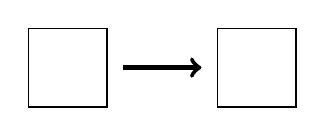
\begin{tikzpicture}
        \begin{scope}
            \draw (0,0) rectangle (1,1);
        \end{scope}
        \begin{scope}[xshift=1.2cm]
            \draw[->,ultra thick] (0,0.5) -- (1,0.5);
        \end{scope}
        \begin{scope}[xshift=2.4cm]
            \draw (0,0) rectangle (1,1);
        \end{scope}
    \end{tikzpicture}
    \caption{Multiple scopes in one \emph{tikzpicture} environment.}
    \label{fig:scopes}
\end{figure}


\section{Conclusion}
\lipsum[2-4]

\section*{Acknowledgments}
The authors would like to thank \dots

\appendix

\section{Acronyms}
This is an appendix that uses acronyms like \gls*{cad}.

\section*{References}
\bibliographystyle{elsarticle-num}
\bibliography{references}

\end{document}
